
The following chapter describes the analysis with two same sign \hadtau and two jets performed with 8\tev data. After a brief description of the data and Monte Carlo samples, details follow on the selection used following the strategy suggested in Chapter \ref{sec:VBFSUSY}. The next section motivates and describes the data-driven background estimation technique used for treating QCD background events where two jets get mis-reconstructed as \hadtau and pass the event selection. The validation of the background estimation method is described in the final section.

\section {Data sample and trigger paths}

The analysis is performed using data collected with the CMS detector
in proton-proton collisions at a centre of mass energy of \CM = 8\tev at the LHC. The data samples correspond to an integrated luminosity of \lumiOld. 

Even though the analysis original concept was relying on the usage of a VBF-based trigger for an online selections on the kinematic properties of the di-jet system resulting from the VBF processes the only unprescaled available alternative is the \texttt{HLT\_\-DoubleMedium\-IsoPFTau35\_\-Trk*\_\-eta2p1\_\-Prong1\_\-v*} trigger. This trigger is the least competitive among all the lepton trigger but is the one with the highest signal acceptance for the \hadtau channel.

\section{Signal and background samples}

%TODO you need to explain more precisely where MC is used: signal prediction, *part* of the bkg prediction, optimization, design of QCD background prediction

%TODO you use “normalize” for 2 different things. Rephrase to make clear  - that you *normalize* the MC yields to the integrated luminosity of the data (quote number) - *by using* cross sections predicted with …  

All the background yields, except for QCD, are taken from simulation. Simulated samples of signal and background events are generated using Monte Carlo (MC) event generators.

The signal event samples are generated with the \texttt{MadGraph v5.1.5} program \cite{Alwall:2011uj}, considering pair production of gauginos with two associated partons. The signal events are generated requiring a pseudorapidity gap $|\deltaeta| > 4.2$ between the two partons, with $\pt > 30\gev$ for each parton. Signal cross sections are calculated at leading order using the MadGraph generator. The range of signal cross sections is $50^{–1}$ fb for \charginopm = \neutralinotwo masses of 100, 200 and 300\gev.

Background event samples with a Higgs boson produced through VBF processes, and single top are generated with the \texttt{POWHEG v1.0r1380} program \cite{Frixione:2007vw}. 
The \texttt{MadGraph v5.1.3} generator is used to describe Z+jets, W+jets, tt, di-boson, and VBF Z boson production. The MC background and signal yields are normalized to the integrated luminosity of the data. 
The \ttbar background is normalized to the next-to-next-to-leading-logarithm level using the calculations presented in references \cite{Czakon:2013goa,Melnikov:2006kv}. 
The Z+jets and W+jets processes are normalized to next-to-next-to-leading-order using the results from the \texttt{FEWZ v2.1} \cite{Gavin:2010az} generator. 
The di-boson background processes are normalized to next-to-leading-order using the \texttt{MCFM v5.8} \cite{Campbell:2010ff} generator, while the VBF Z boson events are normalized to next-to-leading order using the \texttt{VBFNLO v2.6} \cite{Arnold:2008rz,Arnold:2011wj}program. 
The single-top and VBF Higgs boson background yields are taken from the powheg program, where the next-to-leading order effects are incorporated.

All MC samples incorporate the \texttt{CTEQ6L1} \cite{Pumplin:2002vw} or \texttt{CTEQ6M} \cite{Nadolsky:2008zw} parton distribution functions (PDF). The corresponding evaluation of uncertainties in the signal cross sections is discussed in Section \ref{sec:systematics}. The \texttt{POWHEG} and \texttt{MadGraph} generators are interfaced with the \texttt{PYTHIA v6.4.22} \cite{Sjostrand:2006za} program, which is used in the mathing between the matrix elements and the parton shower, and the hadronization processes. 


The decays of $\tau$ leptons are simulated using the \texttt{tauola (27.1215)} \cite{Davidson:2010rw} program. The background samples are processed with a detailed simulation of the CMS apparatus using the \texttt{Geant4} package \cite{Agostinelli:2002hh}, while the response for signal samples is modeled with the CMS fast simulation program \cite{Abdullin:2011zz}. For the signal acceptance and \mjj shapes based on the fast simulation, the differences with respect to the \texttt{Geant4}-based results are found to be small ($< 5\%$). Corrections are applied to account for the differences. 

For all MC samples, multiple proton-proton interactions are superimposed on the primary collision process, and events are reweighted such that the distribution of reconstructed collision vertices matches that in data. The distribution of the number of pileup interactions per event has a mean of 21 and a root-mean-square of 5.5. 

For all datasets, a common \texttt{Physics Analysis Toolkit} (\texttt{PAT}) \cite{Adam:2010zza} sequence has been used to generate samples in PAT format, then further reduced them in size with the ntuple producer \cite{bib:thentuplemaker}.

%TODO how is the trigger modeled in MC? you use the same reconstruction software on MC as on data? 

%TODO (LOW PRIORITY) geant4 is not the full story: electronics and propagation of light through material is emulated (digitization step)(check recent CMS papers)

\section{Event Selection}
\label{sec:eventselection}

%TODO one topic per paragraph

%TODO read it again and try to make your text easier to understand for a reader that is less familiar with LHC analyses

As mentioned in Section \ref{section::search_strategy} the di-\hadtau channel's main background contribution comes from QCD multijetevents, with a rate several orders of magnitude larger than the rate of other background contributions. Hence this search channel, more than any of the other lepton channels, relies on the efficient background rejection. Fortunately, the VBF and \met selections provide the required background suppression.

All the collision data events passing the requirements of the triggers shown in Table \ref{table:triggerdefinition} are considered for offline analysis. 

As previously introduced in Section \ref{section::search_strategy}, the event selection criteria is divided in two distinct parts: the central part, which takes into account the LSP and the decay products of the multiple \hadtau, and the VBF part, which cuts on the kinematic properties of the jets coming from a VBF process. 

The main differences with the other VBF SUSY searches with final states including light leptons, are the substantially tighter \hadtau requirements targeting at the suppression of QCD jet background and the looser missing transverse energy (\met) requirement, to recover some of the signal acceptance lost due to the larger discriminator based on isolation $\hadtau$ \pt thresholds needed to stay efficient with respect to the trigger. 

There are some differences this analysis has with the other existing VBF searches with final states to light leptons. The most important ones are the substantially tighter requirements on the \hadtau isolation and \pt, which allows a good QCD background suppression while remaining efficient with the trigger online requirements. However those requirements leads also to a reduction in the signal acceptance, for that reason a looser \met cut is introduced.

The selected events are required to have at least two \hadtau candidates as defined in Section \ref{subsec::objsel_tau}. The reconstruction of more than two \hadtau is constrained by the trigger. The like sign \hadtau candidates with the highest \pt and separated from each other by a minimum \deltar = 0.3 are then chosen to form a di-\hadtau candidate. 
Further, to reduce top pair contamination the event is required not to have any jet identified as a b--quark jet by the b--tagging algorithms using the {\textit combined secondary vertex loose} (CSVL) working point. 

Only jets with \pt $\ge 30\gev$ and separated from the taus in the di--\hadtau pairs by $\Delta R \ge 0.3$ are searched for b--tags. The \pt cut of 30\gev on b-jets (a looser veto requirement than other analyses with light leptons) allows to be more efficient with respect to the signal since the higher \pt threshold on taus reduces the contamination of $t\overline{t}$ to a large extent. Further, the event is required to have at least 30\gev of \met. All the selections described above is what will be referred to as \textit{central selections}.

Subsequently, the following event-wide requirements are imposed. The {\textit {VBF selections}} are imposed by requiring at least two jets as defined in Section \ref{subsec::objsel_jet}. Only jets separated from the leptons in the \hadtau\hadtau pair by $\deltar \ge 0.3$ are considered. All jet candidates passing the above requirements and having $\vert \Delta\eta \vert \ge 4.2$ and $\eta_{1}\cdot\eta_{2} < 0$ are combined to form di-jet candidates. The final and the most important of the requirement is an invariant mass of the di-jet candidate, denoted \mjj, above the threshold of 250\gev. In order to increase the event acceptance the analysis code algorithm takes into account every possible di-jet candidate combination and chooses the one that passes the VBF requirements and has the highest \mjj. 

For better visualization and understanding all the selection criteria are summarized the following way:

%TODO (LOW priority) it’s more elegant to have this in a table instead of a bullet list.

\begin{itemize}
	\item \textbf{Central selection}
	\begin{itemize}
		\item Trigger: \texttt{HLT\_DoubleMediumIsoPFTau35\_Trk*\_eta2p1\_Prong1\_v*}
		\item two one-prong hadronically decaying $\tau$ with $\pt\geq45~$\gev 
		\item $\met > $ 30
		\item at least two jets with $p_{T}^{jet}\geq30~$\gev, $|\eta_{jet}|\leq5$ and loose jetID
		\item $\Delta R(jet,\tau)\geq0.3$
		\item b-tag veto
	\end{itemize}
	\item \textbf{VBF selection}
	\begin{itemize}
		\item $|\Delta\eta(jet,jet)| > 4.2$
		\item $sign(\eta^{jet 1}\cdot\eta^{jet 2})==-1$
		\item $\mjj>250~$\gev
	\end{itemize}
\end{itemize}

%todo (LOW PRIORITY) you need a cutflow table here, and a discussion about how event yields for data and MC samples reduces with cuts.

\clearpage



\section {LS di-Tau Data-Driven QCD background determination} \label{sec:bgestimation}

%TODO improve flow of information, e.g.
%TODO 1. short introduction to the concept
%TODO 2. definition of control regions ( table with event yields)
%TODO 3. assumptions
%TODO 4. the actual method

The QCD background contribution for the like-sign di-\hadtau channel is done using a ABCD data-driven approach. This method consist in  dividing the analyzed data in different exclusive regions, defined by two variables. The first variable is the \hadtau isolation discriminator used in the object reconstruction, namely:
 	
 	%TODO don’t use these funny names here: just use “tight”, “loose” and “medium”, introduced in the object definition, with a reference such that the really interested can find back what you exactly mean. and you have the appendix anyway.
 	
 	\begin{enumerate}
 		\item Tight or T isolated $\hadtau$ for \texttt{byTight\-IsolationMVA3newDMwLT};
 		\item Medium or M isolated $\hadtau$ for \texttt{byMedium\-IsolationMVA3newDMwLT} but failed \texttt{byTight\-IsolationMVA3newDMwLT};
 		\item Loose or L isolated $\hadtau$  for \texttt{byLoose\-IsolationMVA3newDMwLT} but failed \texttt{byTight\-IsolationMVA3newDMwLT} and \texttt{byMedium\-IsolationMVA3newDMwLT}.
 	\end{enumerate}
 	
Each event with a successfully reconstructed LS di-$\hadtau$ pair falls into a exclusive isolation region as shows on Figure \ref{fig:tauisoregions}:
 	
 	\begin{itemize}
 		\item SR or signal region consisting of two tight isolated $\hadtau$;
 		\item 1T or One Tight isolated $\hadtau$ region consisting of one tight isolated $\hadtau$ and an additional medium or loose isolated $\hadtau$;
 		\item AT or Anti Tight isolation region consisting of at least one medium isolated $\hadtau$ and an additional medium or loose isolated $\hadtau$;
 		\item AM or Anti Medium isolation region consisting of two loose isolated $\hadtau$.
 	\end{itemize}
 
 	\begin{figure}[tbh!]
 		\centering
 		\begin{tabular}{cc}
 			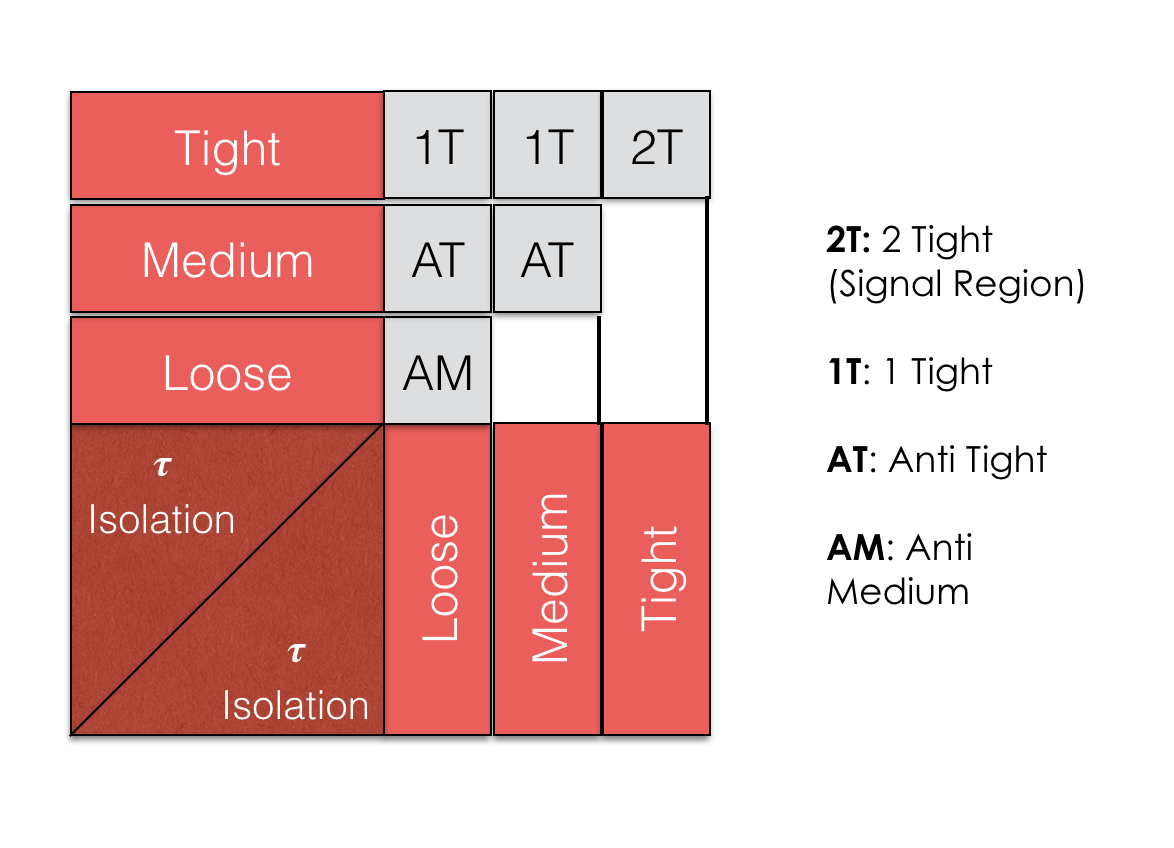
\includegraphics[width=0.75\textwidth]{PLOTS/diTauHadLSotherPlots/tauisoregions.png}
 		\end{tabular}
 		\caption{Definitions of the exclusive isolation region depending on the isolation of each of the $\hadtau$ where SR is Signal Region consisting of two tight isolated $\hadtau$, 1T is One Tight isolated Tau region consisting of one tight isolated $\hadtau$ and an additional medium or loose isolated $\hadtau$, AT is Anti Tight isolation region consisting of at least one medium isolated $\hadtau$ and an additional medium or loose isolated $\hadtau$,  AM is Anti Medium isolation region consisting of two loose isolated $\hadtau$}
 		\label{fig:tauisoregions}
 	\end{figure}
 
The second dimension of exclusivity is based on the VBF cuts described in \ref{sec:eventselection}. The regions are defined the following way:
	
	\begin{enumerate}
		\item VBF region: consisting of all the events that passed all VBF cuts previously mentioned;
		\item VBF inverted region: consisting of all the events that at least fails one of the VBF cuts previously mentioned;
	\end{enumerate} 

Using these definitions one signal region (SR) and seven control regions (CR) are defined as shown in Figure \ref{fig:crs}. The SR falls into the region defined by two tight isolated $\hadtau$ and all the VBF cuts applied, close to it the control region two (CR2) features the same \hadtau isolation requirements but inverted VBF selection requirement. In order to keep the QCD background contribution low in SR and CR2 an additional cut of  \met $ > $ 30\gev is required.

The estimation of the events in the signal region is equivalent to the classic ABCD method consisting in counting the number of events in CR2 and multiplying it with a proper conversion factor. This estimation method has been developed under the following assumptions:

\begin{itemize}
	\item[1] The VBF selection efficiency is independent from any trigger efficiency concerning $\hadtau$ isolation such that each contribution to the numerator and denominator cancels out;
	\item[2] The VBF selection efficiency is also independent from any \met cut applied in order to reduce QCD background contributions. 
\end{itemize}

 The number of   in the following equation:

\begin{equation}
N^{QCD}_{SR} = \left( N^{DATA}_{CR2} - N^{\overline{QCD} BG}_{CR2} \right) * \left[ \frac{\epsilon^{QCD}_{VBF}}{1 - \epsilon^{QCD}_{VBF}} \right]
\label{eq:qcdbgpred}
\end{equation}

where $N^{QCD}_{SR}$ is the number of QCD events predicted in the signal region, $N^{DATA}_{CR2}$ is the number of data events in CR2, $N^{\overline{QCD} BG}_{CR2}$ is the number of all non-QCD MC samples events in CR2 and $\epsilon^{QCD}_{VBF}$ is the efficiency of VBF cuts in a lower \hadtau isolation region. 

Those  control regions are defined as CR3 (One Tight isolation region), CR5  (Anti Tight isolation region) and CR7 (Anti Medium isolation region) followed by their corresponding VBF-inverted control regions CR4, CR6, CR8. An overview of the defined SR and CRs is shown on Figure \ref{fig:crs}. The $\epsilon^{QCD}_{VBF}$ for each of the different \hadtau isolation region is with the following equation.

\begin{figure}[tbh!]
	\centering
	\begin{tabular}{cc}
		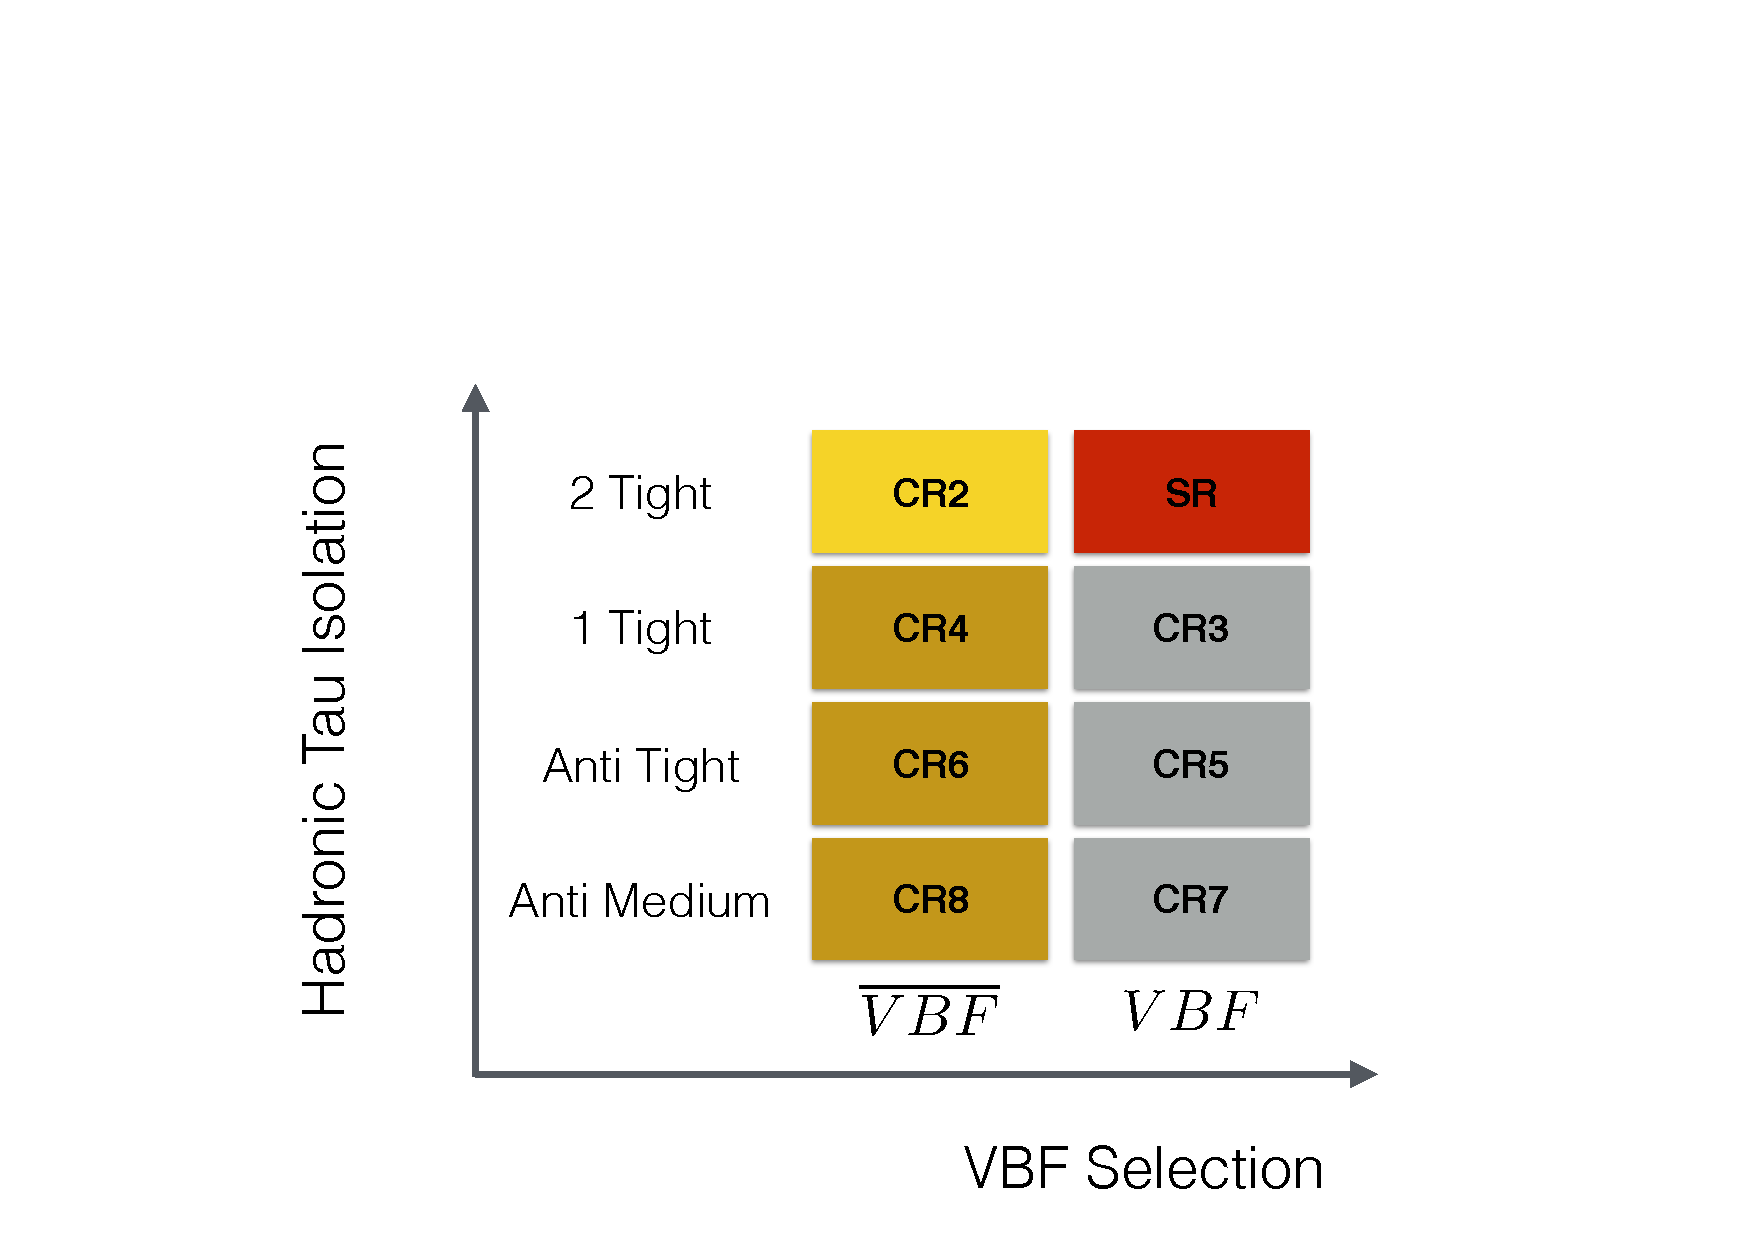
\includegraphics[width=0.75\textwidth]{PLOTS/diTauHadLSotherPlots/controlregions.pdf}
	\end{tabular}
	\caption{Definition of Signal and Control Regions using different $\hadtau$ isolation criteria and VBF selection.}
	\label{fig:crs}
\end{figure}

\begin{equation}
\epsilon^{QCD}_{VBF} = \frac {N^{DATA}_{VBF CR} - N^{\overline{QCD} BG}_{VBFCR}}{\left( N^{DATA}_{VBFCR} - N^{\overline{QCD} BG}_{VBFCR} \right) + \left( N^{DATA}_{\overline{VBF}CR} - N^{\overline{QCD} BG}_{\overline{VBF}CR} \right) }
\label{eq:vbfeff}
\end{equation}

where $N^{DATA}_{VBF CR}$ is the number of the events in data for a given $ \tau $ isolation region and VBF region, $N^{\overline{QCD} BG}_{VBFCR}$ is the number of all non-QCD MC events for a given $ \tau $ isolation region and VBF region, $N^{DATA}_{\overline{VBF}CR}$ is the number of events in data in the same isolation Control Region but inverted VBF region and$N^{\overline{QCD} BG}_{\overline{VBF}CR}$ is the number of all non-QCD MC events for a given $ \tau $ isolation region but inverted VBF region.

Using the events in the defined control regions coming from Table \ref{table:CReventcount} as input for equations \ref{eq:qcdbgpred} and \ref{eq:vbfeff} is possible to determine three different predictions for the QCD background contribution, one for each pair of tau isolation control regions below the two-tight isolation region.

The estimation of the QCD contamination, in the signal region, as shown on Equation \ref{eq:qcdbgpred}, has three sources of systematics. The first source comes from the generated Monte Carlo samples used in the analysis. The two remaining ones comes from the assumptions about the stability of the $\epsilon^{QCD}_{VBF}$, made when defining the data-driven method, one in regard to the relaxation of the tau-identification and the other in regard to a loosening of the \met cut, since the $\epsilon^{QCD}_{VBF}$ is calculated in CRs where no \met cut is applied.

Details and results on the validation process done for all the statements is given in Section \ref{QCD_bg_pred_validation}.

The signal and control regions are define under the assumption of central selection being orthogonal to VBF selection. Figure \ref{fig:LS_mjjshapestab_vs_tauiso_data} and \ref{fig:LS_mjjshapestab_vs_tauiso_mc} shows a stability study of $M_{jj}$ shape distribution among different $\tau$ isolation sidebands for Data and MC. This study shows that within the statistical uncertainties the distributions are compatible for different control regions. Further studies are shown in Section \ref{dihad:tab:stability}.

\begin{figure}[tbh!]
	\centering
	\begin{tabular}{cc}
		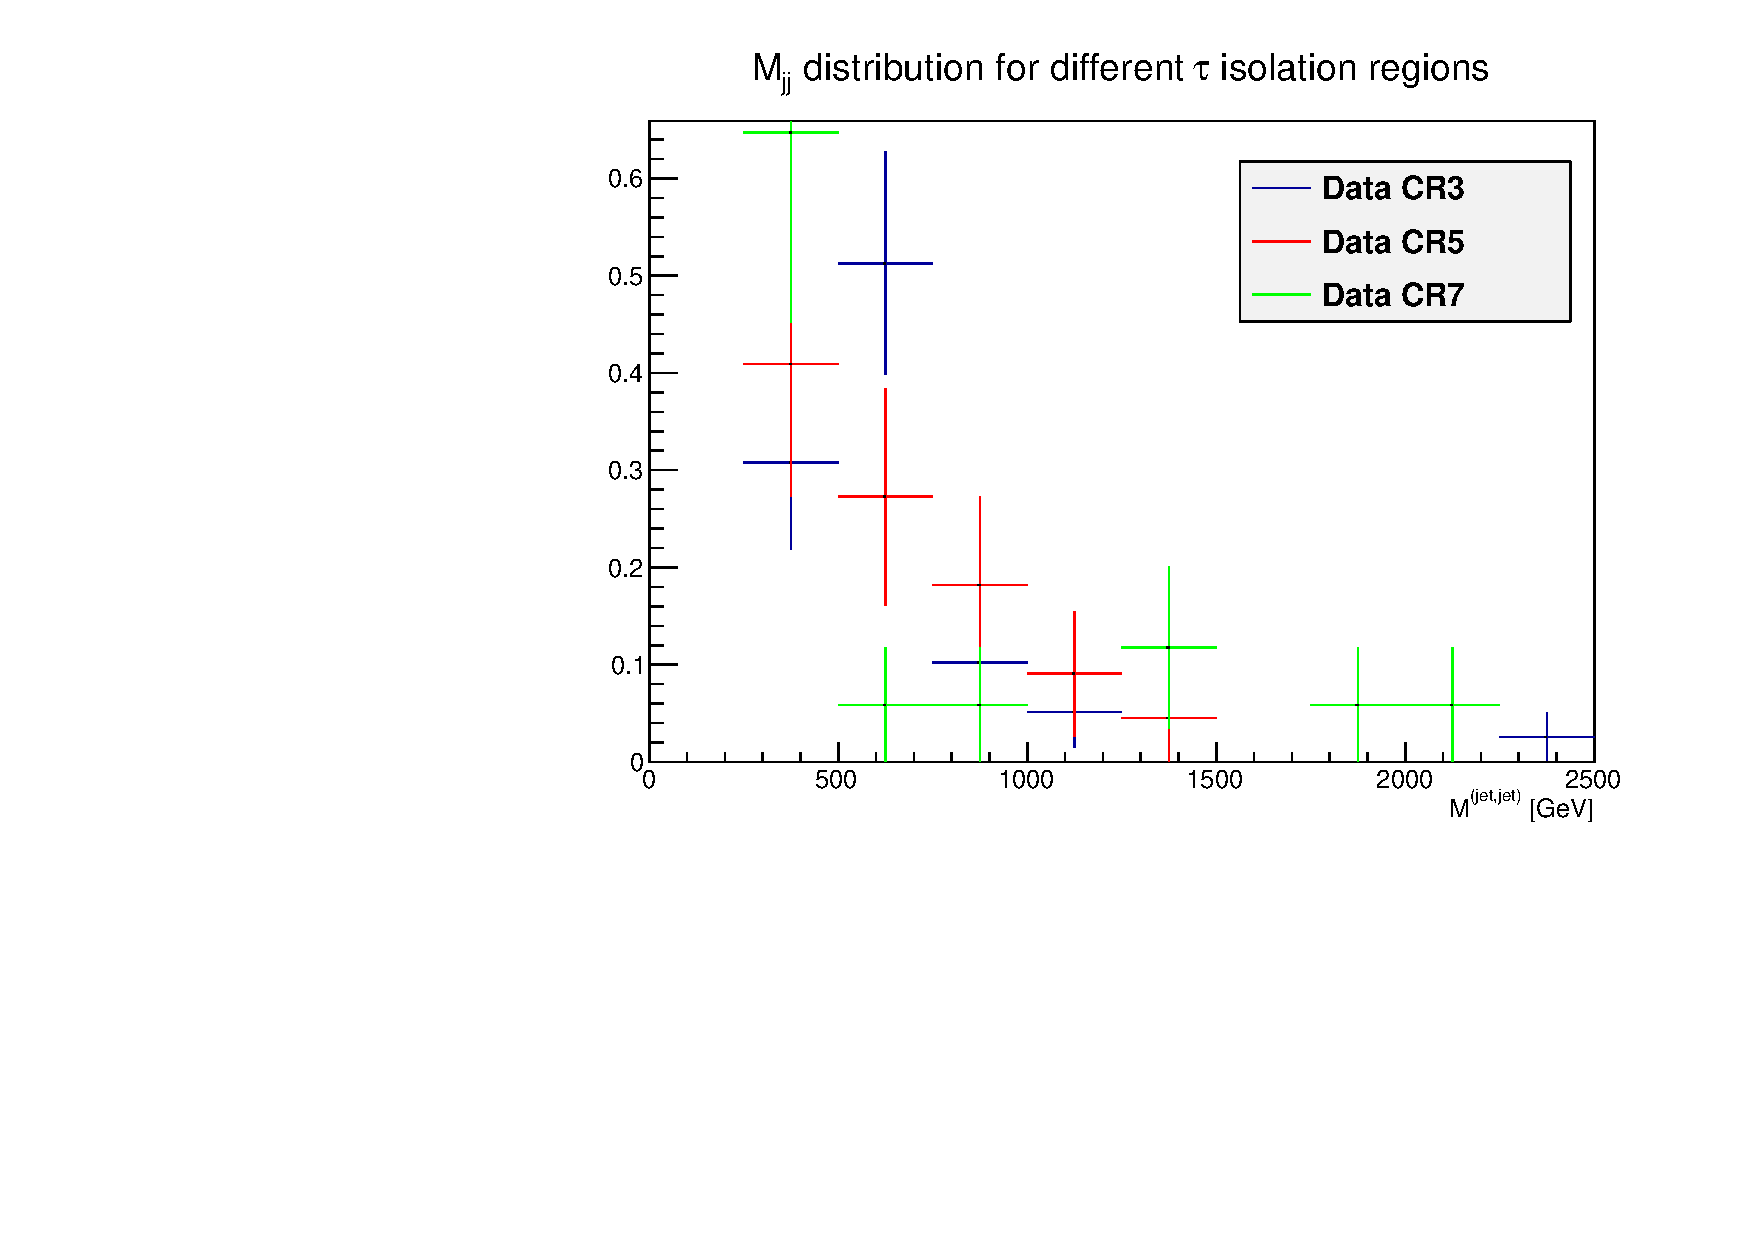
\includegraphics[width=0.75\textwidth]{PLOTS/diTauHadLSotherPlots/LS_mjjshapestab_vs_tauiso_data.pdf}
	\end{tabular}
	\caption{$M_{jj}$ shape comparisons among different $\tau$ isolation sidebands for Data (CR3, CR5, CR7)}
	\label{fig:LS_mjjshapestab_vs_tauiso_data}
\end{figure}

\begin{figure}[tbh!]
	\centering
	\begin{tabular}{cc}
		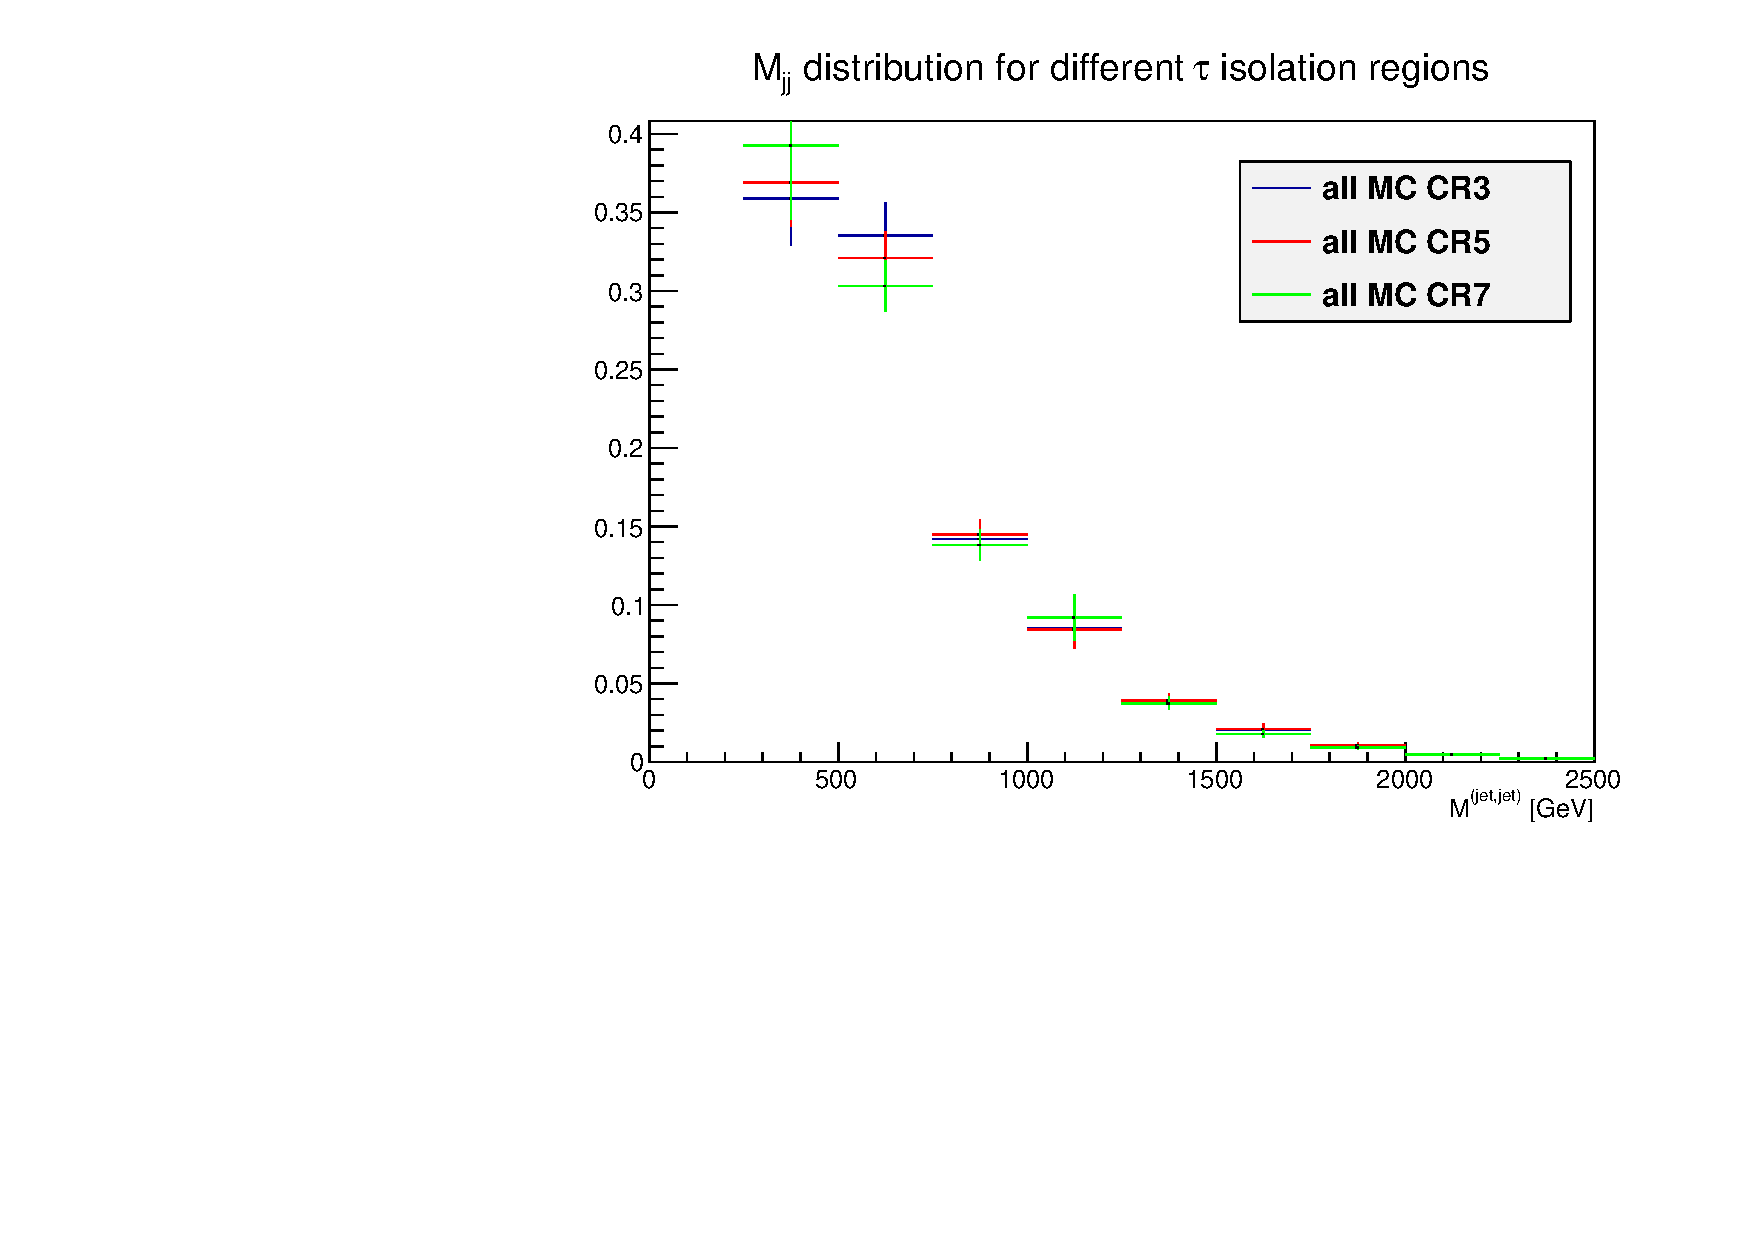
\includegraphics[width=0.75\textwidth]{PLOTS/diTauHadLSotherPlots/LS_mjjshapestab_vs_tauiso_mc.pdf}
	\end{tabular}
	\caption{$M_{jj}$ shape comparisons among different $\tau$ isolation sidebands for all MC contributions (CR3, CR5, CR7)}
	\label{fig:LS_mjjshapestab_vs_tauiso_mc}
\end{figure}

\begin{sidewaystable}
	\centering
	\begin{tabular}{| l | c | c | c | c | c |}
		\hline\hline
		Sample       &Events (CR2)     &Events (CR3)  &Events (CR4)  &Events (CR5)     &Events (CR6)  \\ [0.5ex] \hline
		Data    &$ 109$    &$ 39$   &$ 737$  &$ 22$    &$ 312$  \\
		Drell-Yan    &$ 1.3\pm1$    &$ 0.042\pm0.0077$     &$ 0.65\pm0.045$  &$ 0.002\pm0.00076$    &$ 0.029\pm0.0037$    \\
		VV     &$ 0.7\pm0.09$    &$ 0.035\pm0.017$    &$ 0.6\pm0.1$   &$ 0.0031\pm0.001$    &$ 0.045\pm0.015$   \\
		W+Jets     &$ 6.6\pm0.17$    &$ 0.83\pm0.055$    &$ 10\pm0.2$  &$ 0.081\pm0.0096$    &$ 0.89\pm0.034$      \\
		Single t     &$ 0.25\pm0.017$    &$ 0.057\pm0.008$   &$ 0.47\pm0.02$   &$ 0.011\pm0.00076$   &$ 0.1\pm0.0028$     \\
		\ttbar    &$ 1.4\pm0.051$    &$ 0.19\pm0.013$   &$ 2.5\pm0.059$   &$ 0.04\pm0.0024$    &$ 0.52\pm0.0095$      \\
		Higgs     &$ 0.012\pm0.0048$    &$ 0.0029\pm0.0023$   &$ 0.012\pm0.0044$   &$ 2.7\cdot 10^{-05}\pm1.1\cdot	10^{-05}$    &$ 0.00018\pm2.2\cdot 10^{-05}$   \\
		QCD     &$ 54\pm1.2$    &$ 47\pm1.9$   &$ 3.4\cdot10^{+02}\pm4$  &$ 19\pm0.68$    &$ 1.4\cdot 10^{+02}\pm1.6$    \\
		[0.5ex] \hline
		Total $\overline{QCD}$ MC    &$ 10\pm1$    &$ 1.2\pm0.06$   &$ 15\pm0.24$ &$ 0.14\pm0.01$    &$ 1.6\pm0.038$   \\
		\hline\hline
	\end{tabular}
\caption{Number on events in all the defined control regions for data and all MC samples used for the estimation of $N^{QCD}_{SR}$}
\begin{tabular}{| l | c | c | }
			\hline\hline
Sample      &Events (CR7)     &Events (CR8)  \\ [0.5ex] \hline
Data     &$ 17$    &$ 184 $  \\
Drell-Yan    &$ 0.0012\pm0.00057$    &$ 0.013\pm0.0021 $  \\
VV   &$ 0.0011\pm0.00014$    &$ 0.033\pm0.016 $  \\
W+Jets    &$ 0.036\pm0.0051$    &$ 0.35\pm0.015 $  \\
Single t   &$ 0.0061\pm0.00045$    &$ 0.058\pm0.00087 $  \\
\ttbar  &$ 0.022\pm0.00079$    &$ 0.32\pm0.0054 $  \\
Higgs  &$ 4.9\cdot10^{-06}\pm2.3\cdot 10^{-06}$    &$ 5.7\cdot 10^{-05}\pm1\cdot 10^{-05} $  \\
QCD  &$ 15\pm0.81$    &$ 1.1\cdot 10^{+02}\pm1.7 $  \\
\hline
Total nonQCD MC  &$ 0.067\pm0.0053$    &$ 0.77\pm0.023 $  \\
\hline\hline
\end{tabular}
\label{table:CReventcount}
\end{sidewaystable}

\begin{table}[ht]
	\centering{
		\tabcolsep=0.05cm
		\begin{tabular}{| l | c | c | c |}
			\hline\hline
			Variable     &One Tight region     &Anti-Tight region     &Anti-Medium  \\ [0.5ex] \hline
			$\epsilon^{QCD}_{VBF}$    &$ 0.05\pm0.008 $  &$ 0.066\pm0.014 $  &$ 0.085\pm0.02 $ \\
			$N^{QCD}_{SR}$    &$ 5.2\pm1 $  &$ 6.9\pm1.7 $  &$ 9.1\pm2.5 $ \\
			\hline\hline
		\end{tabular}
	}
	\caption{ Values for $\epsilon^{QCD}_{VBF}$ and $N^{QCD}_{SR}$ for different $ \tau $ isolation regions.}
	\label{table:VBFeffBKGprediction} % is used to refer this table in the text
\end{table}

%TODO replace “systematics” with a more precise description, and motivate the method.

A more precise description for the simulation are estimated by scaling non-QCD contributions by $\pm50~\%$. A systematic error on $\epsilon^{QCD}_{VBF}$ is assigned by using the maximal variation among all $\epsilon^{QCD}_{VBF}$ measurements in different $\tau$ isolation regions with respect to its weighted mean. Similar procedure is done for the assignation of the $\epsilon^{QCD}_{VBF}$ coming from \met cut stability. All the statistical uncertainties are propagated accordingly. Table \ref{table:CReventcount} shows the event counting for all the control regions previously defined for data and all MC samples. All the numbers except the ones coming from the QCD sample are used as input for the QCD background estimation method. For each of the three different $\tau$ isolation regions out of the signal region (1T, AT, AM) an independent measurements of $\epsilon^{QCD}_{VBF}$  and prediction for $N^{QCD}_{SR}$ is made. Due to low statistics in the $\tau$ isolation sidebands the final results will include uncertainties coming from the $\epsilon^{QCD}_{VBF}$ stabilities studies on MC shown in section \ref{subsec:stability}.

\clearpage

\section{Data Driven method validation}
\label{QCD_bg_pred_validation}

The data-driven background estimation method, as previously shown, offered a possibility to circumvent the scarce statistics of the simulated QCD samples. The results given in \autoref{section:results} can be backed by a simulation based approach which come with two main advantages. First this approach can confirm the assumption made for the data-driven method which states that all control regions and the signal region are indeed dominated by QCD events. Second this approach can show that VBF efficiency $\epsilon^{QCD}_{VBF}$ defined in \autoref{eq:vbfeff} is independent, within the systematic uncertainty, with respect to a selection over \met or \hadtau transverse momentum. This section will give a brief description and results of this simulation based approach as shown in the contribution done by one of the previous members of the University of Hamburg research group working on the same analysis \cite{bib:phdthesis:denis}.

\subsection{The simulation-based method}

A solution to the scarce statistics of the QCD sample in the signal region can be solved by taking all the events with at least four reconstructed jets and properly reweighting each one of them. This weight is a function of the probabilities that two of those four reconstructed jets will fake an \hadtau:

\begin{equation}
w^{TT}_{\text{event}} = \sum_{i=0}^{N}P(\text{iso}\mid \text{jet}_{i})\left(\sum_{j=0; j\neq i}^{N}P(\text{iso}\mid \text{jet}_{j})\left[\prod_{k=0; k\neq i,j}^{N}(1-P(\text{iso}\mid \text{jet}_{k}))\right]\right)
\end{equation}

where $P(\text{iso}\mid \text{jet})$ is the probability for a given jet to fake an \hadtau with a given isolation:

\begin{equation}
P(\text{iso}\mid \text{jet}_{i}) = P(\text{iso ID}\mid \text{jet}_{i}) \cdot P(\pt^{\hadtau(\text{fake})} > 45\gev\mid \text{jet}_{i}) \dot \epsilon^{\text{trigger}}(\text{ID})
\end{equation}

where $P(\text{iso ID}\mid \text{jet}_{i})$ is the probability for a given jet to fake a \hadtau with a given TauID selection besides the \pt requirement, $P(\pt^{\hadtau(\text{fake})} > 45\gev\mid \text{jet}_{i})$ is the probability for a given jet reconstructed as fake-\hadtau to pass the requirement of $\pt(\hadtau)> 45\gev$ and $\epsilon^{\text{trigger}}(\text{ID})$ is the efficiency of the trigger ,the one used in the analysis, in selecting events with at least four jets.

$P(\text{iso ID}\mid \text{jet}_{i})$ 

\begin{itemize}
	\item Selection acceptance: the jet pt does not translate directly to hadtau pt, a correction factor is needed to correct the pt of the fake hadtaus.
	\item parametrization for fake probabilities
	\item Trigger acceptance correction
	\item Fixation of fake \hadtau mass
\end{itemize}

\subsection{$\epsilon^{VBF}$-stability with regard to $\tau_{h}$-isolation and $E_{T}^{miss}$-cuts}\label{dihad:subsec:stability}
To test the stability and estimate the systematics, we determine on the diced MC all possible efficiencies of $\epsilon^{VBF}$ in all even and odd control region pairs for a range of $E_{T}^{miss}$-cuts in table \ref{dihad:tab:stability}.
\begin{table}[!h]
	\centering
	\begin{tabular}{|c||c|c|c|}
		\hline
		region     & $\epsilon^{VBF}(E_{T}^{miss}\geq0)$ [$\%$]& $\epsilon^{VBF}(E_{T}^{miss}\geq10)$ [$\%$]& $\epsilon^{VBF}(E_{T}^{miss}\geq20)$ [$\%$]\\ \hline \hline
		LS SR/CR2  & $12.78\pm0.53$ & $12.91\pm0.58$ & $13.06\pm0.67$ \\ \hline
		LS CR3/CR4 & $12.20\pm0.43$ & $12.48\pm0.47$ & $12.46\pm0.53$ \\ \hline
		LS CR5/CR6 & $11.61\pm0.41$ & $11.93\pm0.45$ & $11.91\pm0.50$ \\ \hline
		LS CR7/CR8 & $12.10\pm0.60$ & $12.44\pm0.66$ & $12.75\pm0.83$ \\ \hline \hline
		OS SR/CR2  & $11.46\pm0.72$ & $11.74\pm0.80$ & $12.23\pm1.04$ \\ \hline
		OS CR3/CR4 & $10.62\pm0.31$ & $10.66\pm0.33$ & $10.85\pm0.36$ \\ \hline
		OS CR5/CR6 & $10.98\pm0.48$ & $11.09\pm0.52$ & $11.59\pm0.67$ \\ \hline
		OS CR7/CR8 & $10.67\pm0.36$ & $10.61\pm0.37$ & $11.12\pm0.47$ \\ \hline \hline
		WAM        & $11.33\pm0.15$ & $11.43\pm0.16$ & $11.66\pm0.19$ \\ \hline
		\hline
		\hline
		region     & $\epsilon^{VBF}(E_{T}^{miss}\geq30)$ [$\%$]& $\epsilon^{VBF}(E_{T}^{miss}\geq40)$ [$\%$]& $\epsilon^{VBF}(E_{T}^{miss}\geq50)$ [$\%$]\\ \hline \hline
		LS SR/CR2  & $13.76\pm0.89$ & $14.99\pm1.49$ & $18.09\pm2.93$ \\ \hline
		LS CR3/CR4 & $13.18\pm0.68$ & $14.54\pm1.11$ & $16.58\pm2.08$ \\ \hline
		LS CR5/CR6 & $12.20\pm0.56$ & $13.06\pm0.84$ & $13.34\pm1.12$ \\ \hline
		LS CR7/CR8 & $14.05\pm1.25$ & $15.93\pm2.19$ & $19.26\pm4.14$ \\ \hline \hline
		OS SR/CR2  & $13.14\pm1.58$ & $16.04\pm2.98$ & $21.23\pm6.13$ \\ \hline
		OS CR3/CR4 & $11.08\pm0.41$ & $12.61\pm0.69$ & $14.45\pm1.23$ \\ \hline
		OS CR5/CR6 & $12.19\pm0.95$ & $14.38\pm1.70$ & $18.22\pm3.42$ \\ \hline
		OS CR7/CR8 & $11.37\pm0.54$ & $13.01\pm0.90$ & $14.76\pm1.62$ \\ \hline \hline
		WAM        & $11.98\pm0.23$ & $13.43\pm0.39$ & $14.85\pm0.65$ \\ \hline
	\end{tabular}
	\caption{Stability of epsilonVBF in regard to $E_{T}^{miss}$, sign and $\tau_{h}$-isolation. LS and OS regions are slightly correlated. Here, events can be the same, but the chosen jets to fake $\tau_{h}$ must differ. For efficiencies of one sign, efficiencies are expected to be highly correlated. This is not accounted for in the weighted arithmetic mean (WAM) values shown.}
	\label{dihad:tab:stability}
\end{table}
We do observe a quadratic dependence on $E_{T}^{miss}$, as seen in fig. \ref{dihad:fig:Stability}.

\begin{figure}[!h]
	\centering
	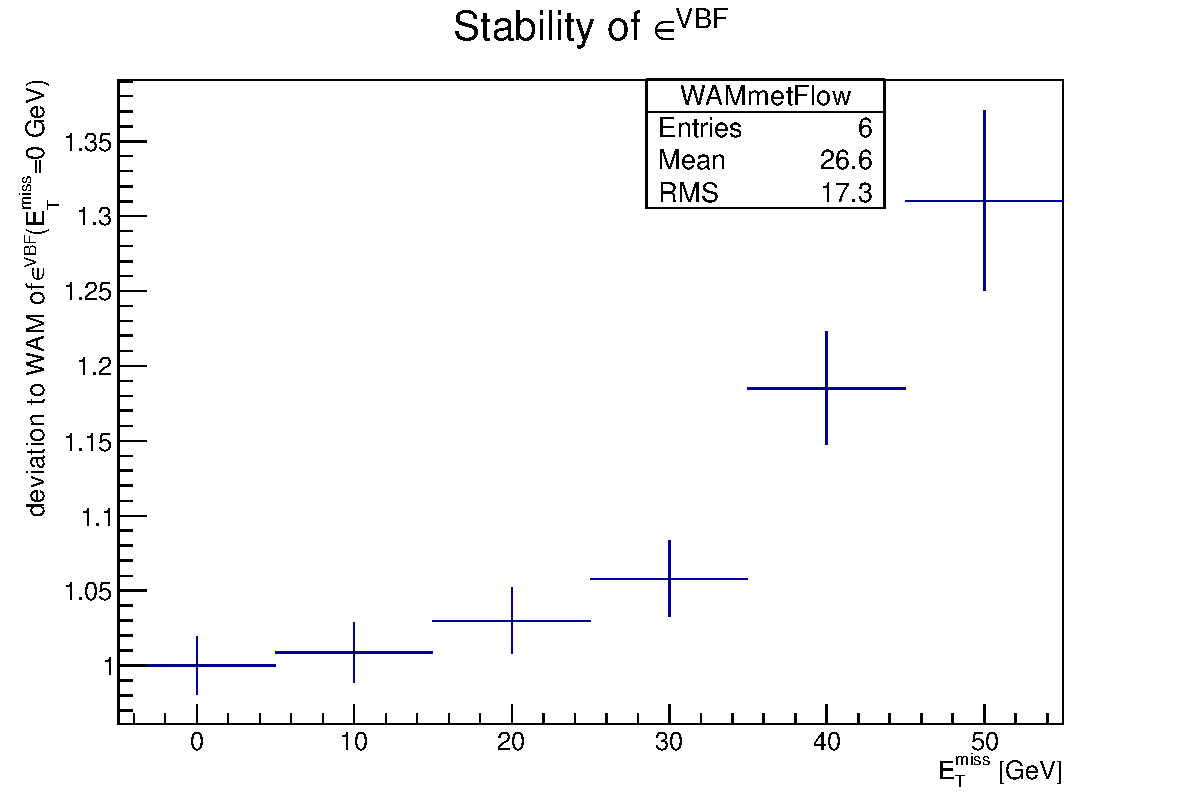
\includegraphics[width=0.5\textwidth]{PLOTS/diTauHadLSQCDPlots/stability/Stability.pdf}
	\caption{\label{dihad:fig:Stability}Deviation of the weighted arithmetic mean (WAM) of the VBF efficiency of all (LS and OS) control region ratios with respect to $E_{T}^{miss}$. We observe a quadratic dependence of small size at the cut-value of 30 GeV we use in this analysis.}
\end{figure}

We derive two systematic errors out of this:
\begin{enumerate}
	\item Stability of $\epsilon^{VBF}$ regarding $\tau_{h}$-isolation: Maximum relative difference to weighted arithmetic mean at $E_{T}^{miss}\geq30$. Amounts to $+17.26\%$ and $-7.58\%$.
	\item Stability of $\epsilon^{VBF}$ regarding $E_{T}^{miss}$-cut: Relative difference to $\epsilon^{VBF}$ within uncertainties of weighted arithmetic
	mean at no cut on $E_{T}^{miss}$ as seen in fig. \ref{dihad:fig:Stability}. Amounts to $+8.30\%$ on the upper edge and $+3.26\%$ on the lower edge.
\end{enumerate}

\clearpage



